% appendix/A-system-screenshots.tex
\chapter{ภาพหน้าจอระบบ (System Screenshots)}
\label{app:screenshots}

ภาคผนวกนี้รวบรวมภาพหน้าจอจากระบบที่พัฒนาขึ้น เพื่อใช้ประกอบการอธิบาย
การทำงานในบทที่ 4. ภาพในภาคผนวกนี้เป็น \emph{ภาพจำลอง UI (UI mockup)}
ที่สร้างจาก TikZ ตามองค์ประกอบจริงของระบบ. ภาพถ่ายจาก production จะถูก
นำมาแทนที่ในการเข้าเล่มฉบับสมบูรณ์ จาก URL
\url{https://construction-cost-engine.steep-tooth-c420.workers.dev}.

\section{หน้าหลัก (Home)}
% figures/screenshot-home.tex — production screenshot of /
\begin{figure}[H]
  \centering
  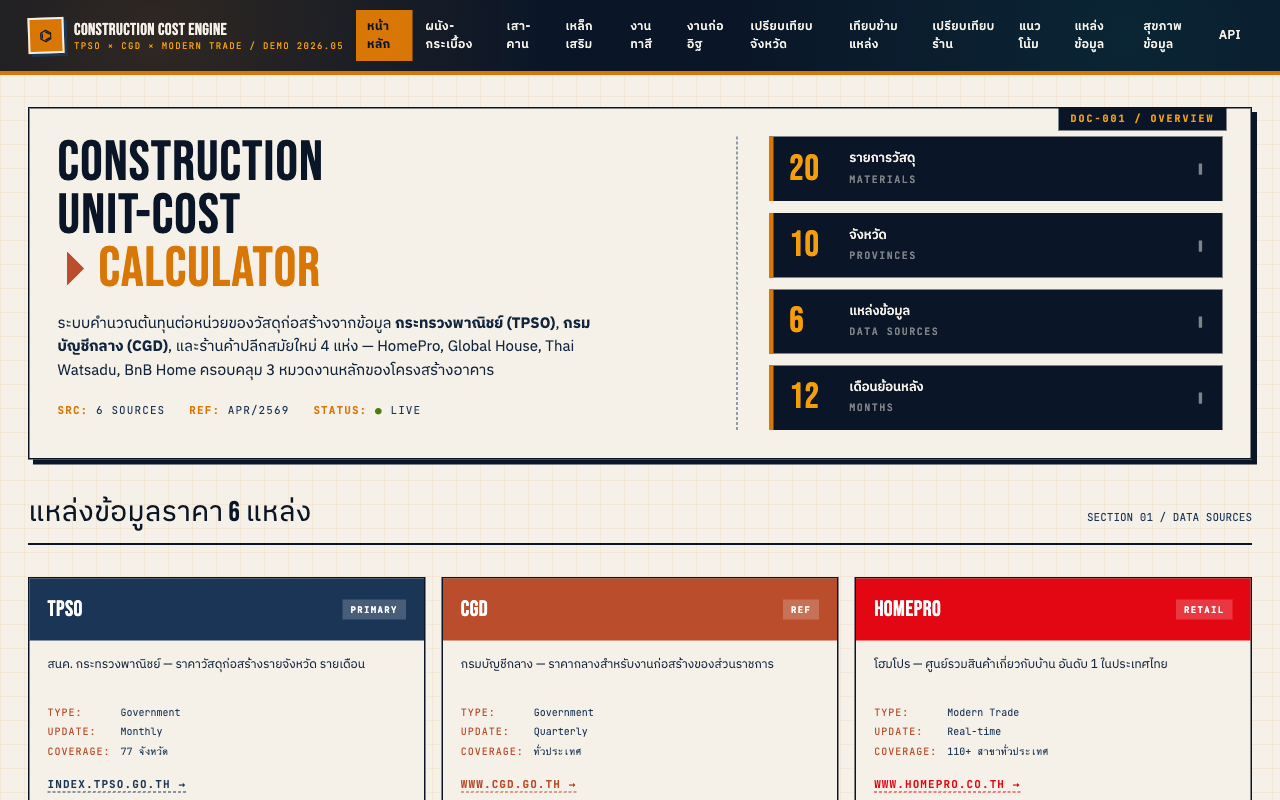
\includegraphics[width=0.95\textwidth]{figures/screen-home.png}
  \caption{หน้าหลัก (\texttt{/}) ของระบบ. แสดงสรุปจำนวนแหล่งข้อมูล รายการวัสดุ พื้นที่ครอบคลุม และทางลัดสู่ฟังก์ชันหลักที่วิศวกรประมาณราคาใช้บ่อยที่สุด.}
  \label{fig:scr-home}
\end{figure}


\section{เปรียบเทียบราคาข้ามแหล่ง (\texttt{/compare-sources})}
% figures/screenshot-compare.tex — production screenshot of /compare-sources
\begin{figure}[H]
  \centering
  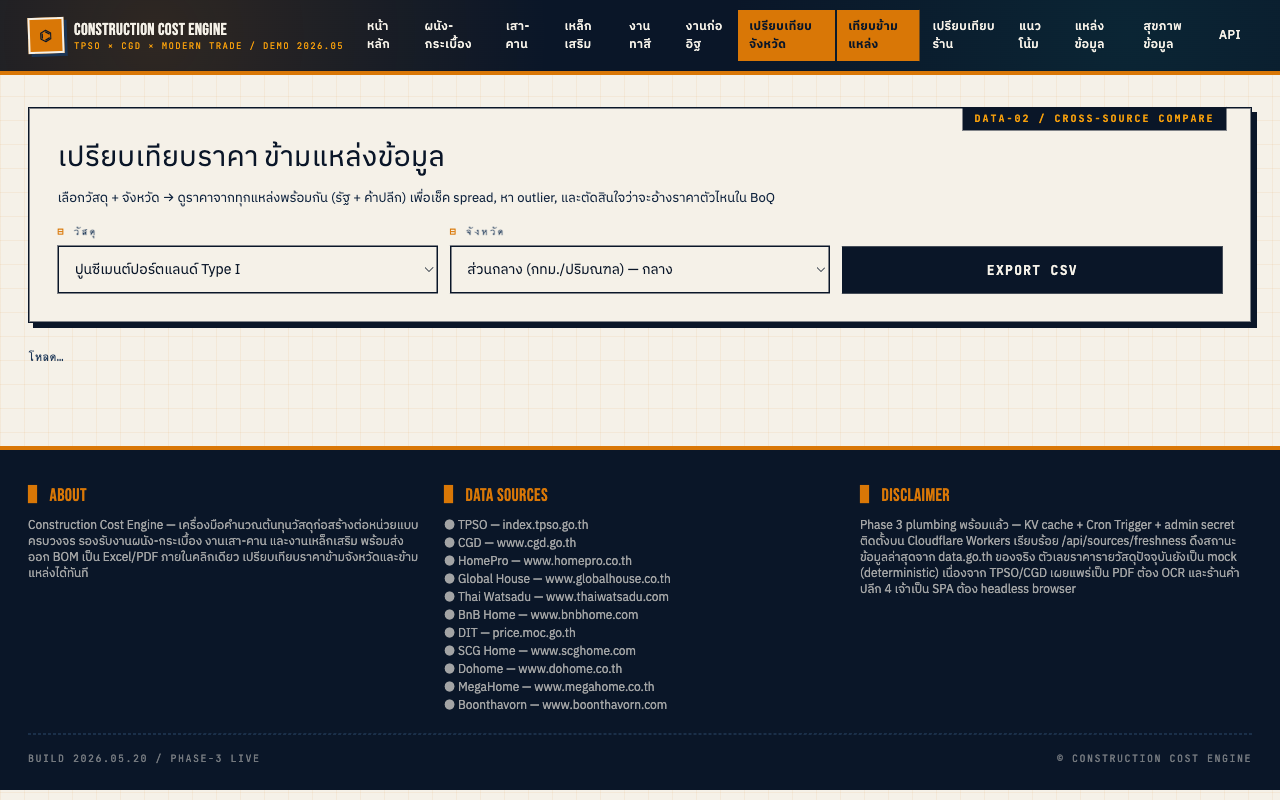
\includegraphics[width=0.95\textwidth]{figures/screen-compare.png}
  \caption{หน้าเปรียบเทียบราคา (\texttt{/compare-sources}). ตารางแสดงราคาเทียบจาก 11 แหล่งข้อมูล ทั้งภาครัฐและภาคค้าปลีกสมัยใหม่ พร้อมเวลา freshness และ flag ราคาที่อาจเป็น outlier.}
  \label{fig:scr-compare}
\end{figure}


\section{แนวโน้มราคา (\texttt{/trend})}
% figures/screenshot-trend.tex — production screenshot of /trend
\begin{figure}[H]
  \centering
  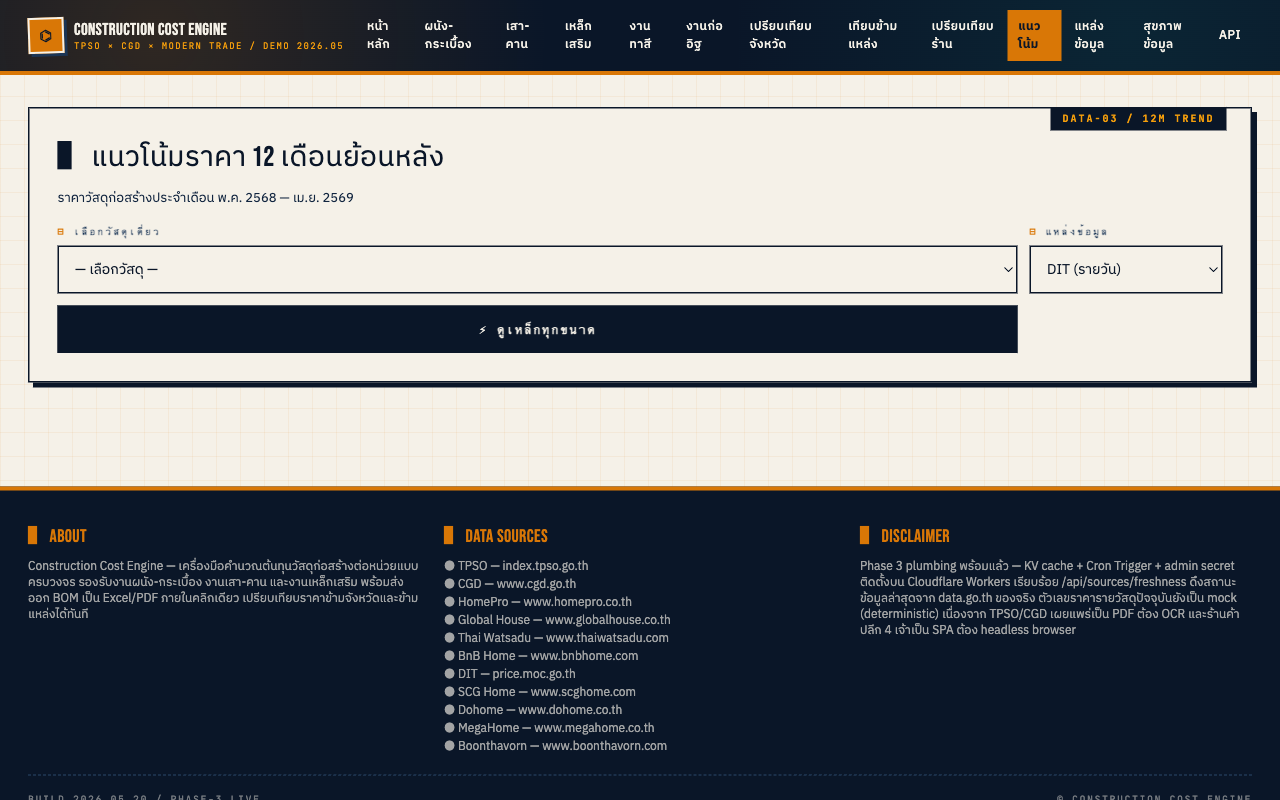
\includegraphics[width=0.95\textwidth]{figures/screen-trend.png}
  \caption{หน้าแนวโน้มราคา (\texttt{/trend}) แสดงดัชนี TPSO CMI 9 เดือน พร้อมเส้นแนวโน้มเชิงเส้น ($R^{2} = 0.989$). ตัวเลขสรุปด้านขวาเป็นข้อมูลที่วิศวกรประมาณราคาใช้เผื่อในงบประมาณโครงการระยะยาว.}
  \label{fig:scr-trend}
\end{figure}


\section{เครื่องคิดเลข BoQ (\texttt{/wall-tile}, \texttt{/paint}, \ldots)}
% figures/screenshot-walltile.tex — UI mockup of /wall-tile (BOQ calculator)
\begin{figure}[H]
  \centering
  \begin{tikzpicture}[font=\scriptsize]
    \draw[draw=gray!50,fill=gray!3,rounded corners=4pt] (0,0) rectangle (12,8);
    \draw[fill=blue!25,draw=blue!50] (0,7.3) rectangle (12,8);
    \node[anchor=west,font=\bfseries] at (0.3,7.65) {คำนวณ BOQ — งานบุกระเบื้องผนัง};

    % Input panel (left)
    \draw[fill=white,draw=gray!50,rounded corners=2pt] (0.3,1.0) rectangle (5.7,7.0);
    \node[anchor=west,font=\bfseries] at (0.5,6.7) {ข้อมูลงาน};
    \node[anchor=west] at (0.5,6.2) {พื้นที่ผนัง (ตร.ม.):};
    \draw[fill=gray!10] (3.0,6.0) rectangle (5.5,6.4); \node[font=\bfseries] at (4.25,6.2) {50};
    \node[anchor=west] at (0.5,5.6) {ขนาดกระเบื้อง:};
    \draw[fill=gray!10] (3.0,5.4) rectangle (5.5,5.8); \node at (4.25,5.6) {30 $\times$ 30 ซม.};
    \node[anchor=west] at (0.5,5.0) {เกรด:};
    \draw[fill=gray!10] (3.0,4.8) rectangle (5.5,5.2); \node at (4.25,5.0) {เกรด A};
    \node[anchor=west] at (0.5,4.4) {ปูนกาว:};
    \draw[fill=gray!10] (3.0,4.2) rectangle (5.5,4.6); \node at (4.25,4.4) {กาวซีเมนต์ 20 กก.};
    \node[anchor=west] at (0.5,3.8) {ภูมิภาค:};
    \draw[fill=gray!10] (3.0,3.6) rectangle (5.5,4.0); \node at (4.25,3.8) {ภาคตะวันออกเฉียงเหนือ};
    \node[anchor=west] at (0.5,3.2) {แหล่งราคา:};
    \draw[fill=gray!10] (3.0,3.0) rectangle (5.5,3.4); \node at (4.25,3.2) {Modern Trade เฉลี่ย};

    \draw[fill=blue!60,draw=blue!80,rounded corners=2pt] (1.0,1.5) rectangle (5.0,2.2);
    \node[white,font=\bfseries] at (3.0,1.85) {คำนวณต้นทุน};

    % Result panel (right)
    \draw[fill=green!5,draw=green!50,rounded corners=2pt] (6.1,1.0) rectangle (11.7,7.0);
    \node[anchor=west,font=\bfseries] at (6.3,6.7) {Bill of Materials};
    \draw[draw=gray!40] (6.3,6.5) -- (11.5,6.5);
    \foreach \i/\m/\q/\u/\p in {
      0/{กระเบื้อง 30$\times$30}/55/แผ่น/{8\,250},
      1/ปูนกาว 20 กก./4/ถุง/{1\,720},
      2/ยาแนว/2/ถุง/{420},
      3/spacer 3 มม./1/ถุง/{180}
    } {
      \node[anchor=west] at (6.3,6.0 - \i*0.45) {\m};
      \node[anchor=east] at (8.5,6.0 - \i*0.45) {\q};
      \node[anchor=west,gray!70] at (8.6,6.0 - \i*0.45) {\u};
      \node[anchor=east,font=\bfseries] at (11.5,6.0 - \i*0.45) {\p};
    }
    \draw[draw=gray!40] (6.3,3.9) -- (11.5,3.9);
    \node[anchor=west,font=\bfseries] at (6.3,3.6) {รวมต้นทุนวัสดุ};
    \node[anchor=east,font=\bfseries] at (11.5,3.6) {10\,570 บาท};
    \node[anchor=west,gray!70,font=\scriptsize] at (6.3,3.2) {ราคาเฉลี่ย/ตร.ม.};
    \node[anchor=east,font=\bfseries,gray!70] at (11.5,3.2) {211 บาท};

    % Export buttons
    \draw[fill=gray!20,draw=gray!50,rounded corners=2pt] (6.3,1.4) rectangle (8.3,2.0);
    \node[font=\scriptsize\bfseries] at (7.3,1.7) {Export Excel};
    \draw[fill=gray!20,draw=gray!50,rounded corners=2pt] (8.6,1.4) rectangle (10.6,2.0);
    \node[font=\scriptsize\bfseries] at (9.6,1.7) {Export PDF};
  \end{tikzpicture}
  \caption{หน้าคำนวณ BOQ งานบุกระเบื้องผนัง (\texttt{/wall-tile}). ผู้ใช้ป้อนพื้นที่งาน ขนาดกระเบื้อง และเลือกแหล่งราคา ระบบจะคำนวณ Bill of Materials ตามหลักเกณฑ์การคำนวณราคากลางของกรมบัญชีกลาง พร้อมรองรับการ export เป็น Excel/PDF เพื่อใช้ในเอกสารโครงการ.}
  \label{fig:scr-walltile}
\end{figure}


\section{สุขภาพแหล่งข้อมูล (\texttt{/health})}
% figures/screenshot-health.tex — UI mockup of /health (system status)
\begin{figure}[H]
  \centering
  \begin{tikzpicture}[font=\scriptsize]
    \draw[draw=gray!50,fill=gray!3,rounded corners=4pt] (0,0) rectangle (12,7.5);
    \draw[fill=blue!25,draw=blue!50] (0,6.8) rectangle (12,7.5);
    \node[anchor=west,font=\bfseries] at (0.3,7.15) {สถานะระบบ — System Health};

    % Overall status badge
    \draw[fill=green!30,draw=green!60,rounded corners=4pt] (0.3,5.9) rectangle (3.5,6.5);
    \node[font=\bfseries] at (1.9,6.2) {\textcolor{green!50!black}{$\bullet$ ปกติ (Healthy)}};

    % Stats summary row
    \foreach \x/\v/\l in {0.3/9/{แหล่ง online}, 3.2/2/{แหล่ง degraded}, 6.1/0/{แหล่ง offline}, 9.0/4.7\%/{outlier rate}} {
      \draw[fill=white,draw=gray!40,rounded corners=2pt] (\x,4.9) rectangle (\x+2.7,5.6);
      \node[font=\bfseries] at (\x+1.35,5.35) {\v};
      \node[font=\scriptsize,gray!70] at (\x+1.35,5.05) {\l};
    }

    % Per-source table
    \node[anchor=west,font=\bfseries] at (0.3,4.5) {รายแหล่ง (cron job last run)};
    \draw[fill=gray!15] (0.3,3.95) rectangle (11.7,4.3);
    \node[anchor=west,font=\bfseries] at (0.5,4.13) {Source};
    \node[anchor=west,font=\bfseries] at (4.0,4.13) {Status};
    \node[anchor=west,font=\bfseries] at (6.5,4.13) {Last update};
    \node[anchor=west,font=\bfseries] at (9.5,4.13) {Records};

    \foreach \i/\src/\st/\time/\rec/\c in {
      0/TPSO/{$\bullet$ ok}/{2 ชม.}/{216}/green,
      1/CGD/{$\bullet$ ok}/{6 ชม.}/{ 24}/green,
      2/DIT/{$\bullet$ ok}/{24 ชม.}/{ 18}/green,
      3/HomePro/{$\bullet$ ok}/{1 ชม.}/{120}/green,
      4/MegaHome/{$\bullet$ ok}/{1 ชม.}/{ 96}/green,
      5/บุญถาวร/{$\bullet$ ok}/{2 ชม.}/{ 48}/green,
      6/ไทวัสดุ/{$\bullet$ ok}/{2 ชม.}/{ 72}/green,
      7/โกลบอลเฮ้าส์/{$\bullet$ degraded}/{14 ชม.}/{ 18}/orange!50!black,
      8/ดูโฮม/{$\bullet$ ok}/{3 ชม.}/{ 24}/green,
      9/เอสซีจีโฮม/{$\bullet$ ok}/{1 ชม.}/{ 12}/green,
      10/บีเอ็นบีโฮม/{$\bullet$ degraded}/{18 ชม.}/{  6}/orange!50!black
    } {
      \node[anchor=west] at (0.5,3.7 - \i*0.30) {\src};
      \node[anchor=west,\c] at (4.0,3.7 - \i*0.30) {\st};
      \node[anchor=west] at (6.5,3.7 - \i*0.30) {\time};
      \node[anchor=west,font=\ttfamily] at (9.5,3.7 - \i*0.30) {\rec};
    }
  \end{tikzpicture}
  \caption{หน้า \texttt{/health} แสดงสถานะระบบและความสดของข้อมูลแต่ละแหล่ง. คอลัมน์ ``Last update'' เป็นข้อมูลที่วิศวกรประมาณราคาใช้ตัดสินว่าราคาในระบบปัจจุบันเชื่อถือได้สำหรับโครงการเร่งด่วนหรือไม่ — แหล่งที่ \texttt{degraded} จะแสดงราคาล่าสุดที่ดึงสำเร็จพร้อม timestamp.}
  \label{fig:scr-health}
\end{figure}

